\documentclass[14pt]{extbook}
\usepackage{multicol, enumerate, enumitem, hyperref, color, soul, setspace, parskip, fancyhdr} %General Packages
\usepackage{amssymb, amsthm, amsmath, bbm, latexsym, units, mathtools} %Math Packages
\everymath{\displaystyle} %All math in Display Style
% Packages with additional options
\usepackage[headsep=0.5cm,headheight=12pt, left=1 in,right= 1 in,top= 1 in,bottom= 1 in]{geometry}
\usepackage[usenames,dvipsnames]{xcolor}
\usepackage{dashrule}  % Package to use the command below to create lines between items
\newcommand{\litem}[1]{\item#1\hspace*{-1cm}\rule{\textwidth}{0.4pt}}
\pagestyle{fancy}
\lhead{Makeup Progress Quiz 1}
\chead{}
\rhead{Version B}
\lfoot{6018-3080}
\cfoot{}
\rfoot{Spring 2021}
\begin{document}

\begin{enumerate}
\litem{
Graph the equation below.\[ f(x) = (x-2)^2 - 19 \]\begin{enumerate}[label=\Alph*.]
\begin{multicols}{2}\item 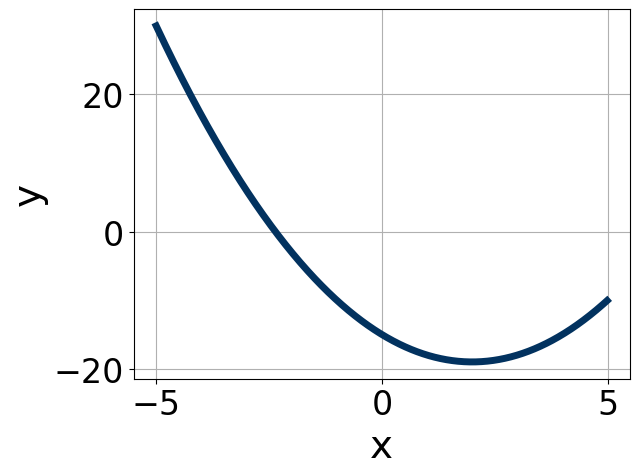
\includegraphics[width = 0.3\textwidth]{../Figures/quadraticEquationToGraphAB.png}\item 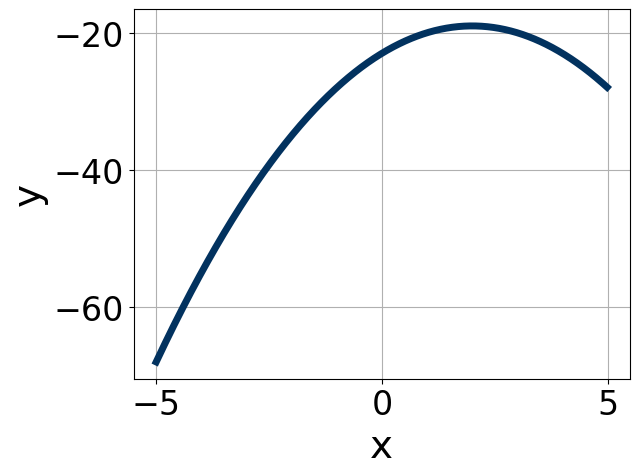
\includegraphics[width = 0.3\textwidth]{../Figures/quadraticEquationToGraphBB.png}\item 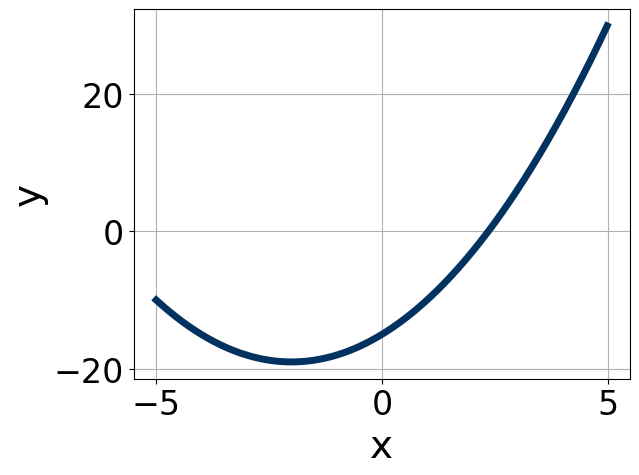
\includegraphics[width = 0.3\textwidth]{../Figures/quadraticEquationToGraphCB.png}\item 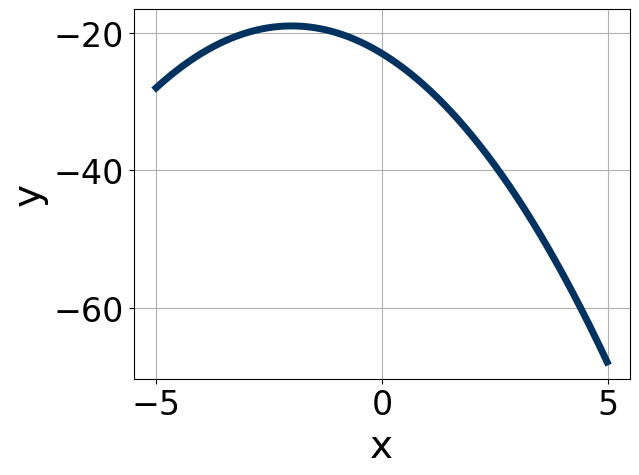
\includegraphics[width = 0.3\textwidth]{../Figures/quadraticEquationToGraphDB.png}\end{multicols}\item None of the above.
\end{enumerate} }
\litem{
Write the equation of the graph presented below in the form $f(x)=ax^2+bx+c$, assuming  $a=1$ or $a=-1$. Then, choose the intervals that $a, b,$ and $c$ belong to.
\begin{center}
    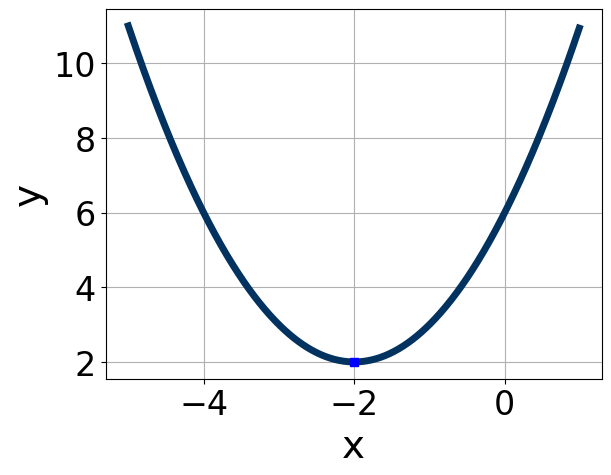
\includegraphics[width=0.5\textwidth]{../Figures/quadraticGraphToEquationCopyB.png}
\end{center}
\begin{enumerate}[label=\Alph*.]
\item \( a \in [-1, 0], \hspace*{5mm} b \in [-5, -3], \text{ and } \hspace*{5mm} c \in [-2, 0] \)
\item \( a \in [1, 2], \hspace*{5mm} b \in [1, 9], \text{ and } \hspace*{5mm} c \in [3, 10] \)
\item \( a \in [1, 2], \hspace*{5mm} b \in [-5, -3], \text{ and } \hspace*{5mm} c \in [1, 4] \)
\item \( a \in [-1, 0], \hspace*{5mm} b \in [1, 9], \text{ and } \hspace*{5mm} c \in [-2, 0] \)
\item \( a \in [1, 2], \hspace*{5mm} b \in [-5, -3], \text{ and } \hspace*{5mm} c \in [3, 10] \)

\end{enumerate} }
\litem{
Solve the quadratic equation below. Then, choose the intervals that the solutions belong to, with $x_1 \leq x_2$ (if they exist).\[ 19x^{2} -10 x -3 = 0 \]\begin{enumerate}[label=\Alph*.]
\item \( x_1 \in [-19.2, -16.3] \text{ and } x_2 \in [18.09, 18.49] \)
\item \( x_1 \in [-0.4, 0.5] \text{ and } x_2 \in [0.51, 1.15] \)
\item \( x_1 \in [-6, -3.7] \text{ and } x_2 \in [13.35, 14.52] \)
\item \( x_1 \in [-1.3, -0.3] \text{ and } x_2 \in [-0.5, 0.37] \)
\item \( \text{There are no Real solutions.} \)

\end{enumerate} }
\litem{
Write the equation of the graph presented below in the form $f(x)=ax^2+bx+c$, assuming  $a=1$ or $a=-1$. Then, choose the intervals that $a, b,$ and $c$ belong to.
\begin{center}
    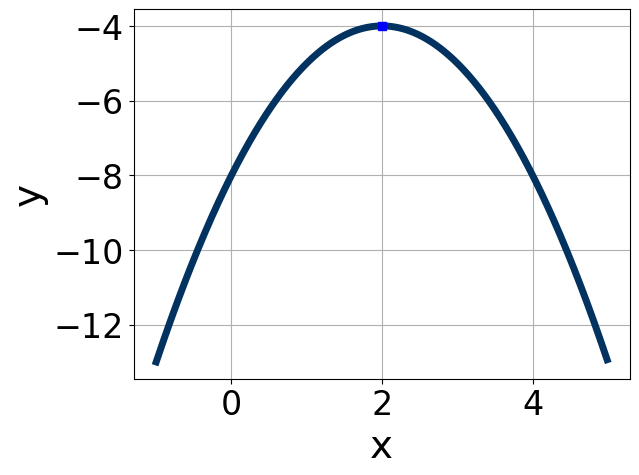
\includegraphics[width=0.5\textwidth]{../Figures/quadraticGraphToEquationB.png}
\end{center}
\begin{enumerate}[label=\Alph*.]
\item \( a \in [-1.8, -0.7], \hspace*{5mm} b \in [-7, 1], \text{ and } \hspace*{5mm} c \in [0, 1] \)
\item \( a \in [0.6, 1.3], \hspace*{5mm} b \in [-7, 1], \text{ and } \hspace*{5mm} c \in [0, 1] \)
\item \( a \in [-1.8, -0.7], \hspace*{5mm} b \in [-7, 1], \text{ and } \hspace*{5mm} c \in [-9, -4] \)
\item \( a \in [-1.8, -0.7], \hspace*{5mm} b \in [1, 7], \text{ and } \hspace*{5mm} c \in [-9, -4] \)
\item \( a \in [0.6, 1.3], \hspace*{5mm} b \in [1, 7], \text{ and } \hspace*{5mm} c \in [0, 1] \)

\end{enumerate} }
\litem{
Solve the quadratic equation below. Then, choose the intervals that the solutions $x_1$ and $x_2$ belong to, with $x_1 \leq x_2$.\[ 25x^{2} +60 x + 36 = 0 \]\begin{enumerate}[label=\Alph*.]
\item \( x_1 \in [-4.82, -2.63] \text{ and } x_2 \in [-0.48, -0.29] \)
\item \( x_1 \in [-6.91, -5.4] \text{ and } x_2 \in [-0.33, -0.22] \)
\item \( x_1 \in [-1.41, -0.49] \text{ and } x_2 \in [-1.26, -1.07] \)
\item \( x_1 \in [-2.76, -2.33] \text{ and } x_2 \in [-0.69, -0.51] \)
\item \( x_1 \in [-30.24, -29.75] \text{ and } x_2 \in [-30.02, -29.88] \)

\end{enumerate} }
\litem{
Graph the equation below.\[ f(x) = (x+1)^2 + 16 \]\begin{enumerate}[label=\Alph*.]
\begin{multicols}{2}\item 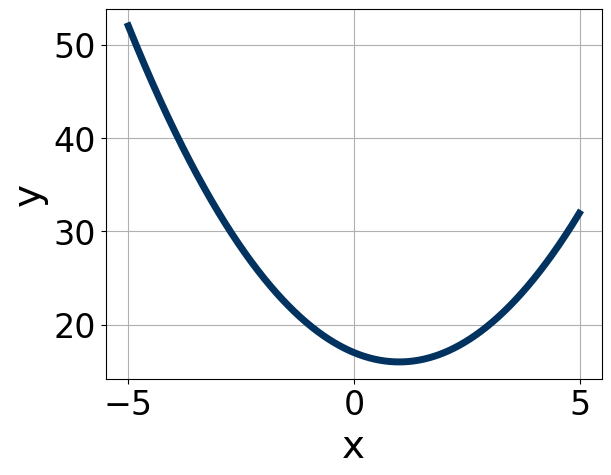
\includegraphics[width = 0.3\textwidth]{../Figures/quadraticEquationToGraphCopyAB.png}\item 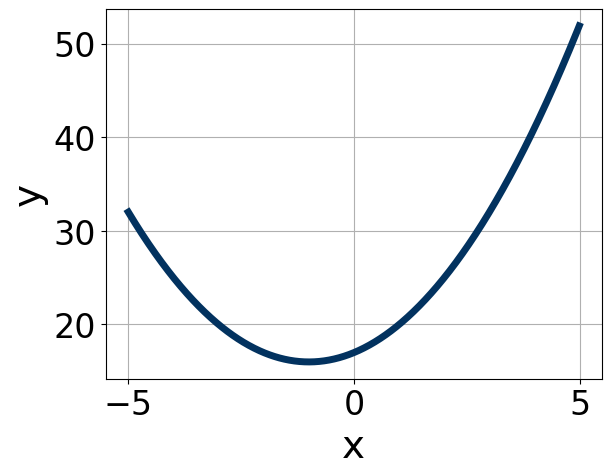
\includegraphics[width = 0.3\textwidth]{../Figures/quadraticEquationToGraphCopyBB.png}\item 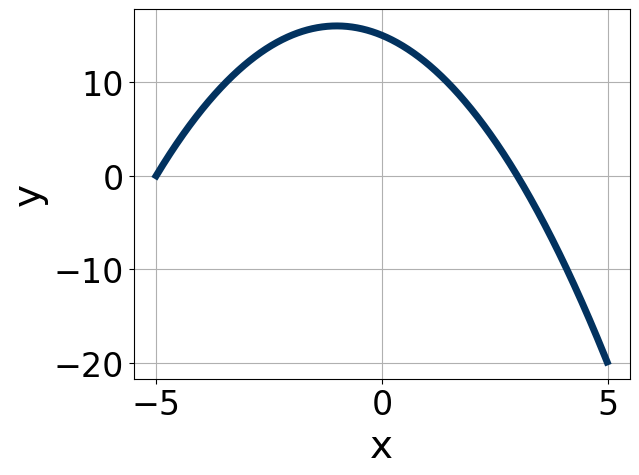
\includegraphics[width = 0.3\textwidth]{../Figures/quadraticEquationToGraphCopyCB.png}\item 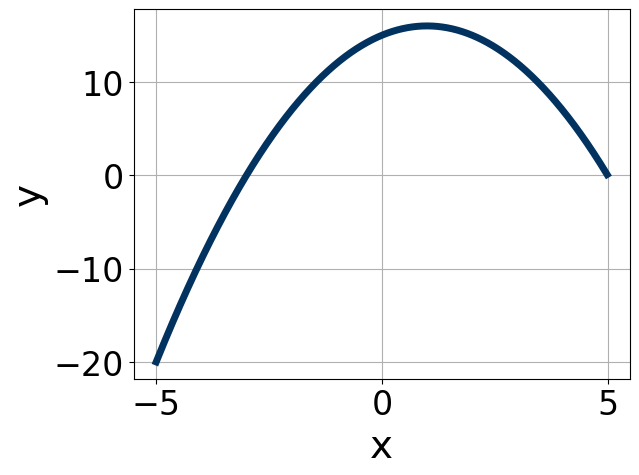
\includegraphics[width = 0.3\textwidth]{../Figures/quadraticEquationToGraphCopyDB.png}\end{multicols}\item None of the above.
\end{enumerate} }
\litem{
Factor the quadratic below. Then, choose the intervals that contain the constants in the form $(ax+b)(cx+d); b \leq d.$\[ 36x^{2} +60 x + 25 \]\begin{enumerate}[label=\Alph*.]
\item \( a \in [16.18, 18.1], \hspace*{5mm} b \in [1, 9], \hspace*{5mm} c \in [1.4, 3.28], \text{ and } \hspace*{5mm} d \in [-1, 9] \)
\item \( a \in [1.52, 3.58], \hspace*{5mm} b \in [1, 9], \hspace*{5mm} c \in [16.37, 19.52], \text{ and } \hspace*{5mm} d \in [-1, 9] \)
\item \( a \in [-0.33, 1.24], \hspace*{5mm} b \in [30, 32], \hspace*{5mm} c \in [0.64, 1.46], \text{ and } \hspace*{5mm} d \in [28, 36] \)
\item \( a \in [5.87, 6.69], \hspace*{5mm} b \in [1, 9], \hspace*{5mm} c \in [5.85, 7.56], \text{ and } \hspace*{5mm} d \in [-1, 9] \)
\item \( \text{None of the above.} \)

\end{enumerate} }
\litem{
Solve the quadratic equation below. Then, choose the intervals that the solutions $x_1$ and $x_2$ belong to, with $x_1 \leq x_2$.\[ 20x^{2} -69 x + 54 = 0 \]\begin{enumerate}[label=\Alph*.]
\item \( x_1 \in [0.41, 0.47] \text{ and } x_2 \in [5.58, 6.54] \)
\item \( x_1 \in [0.73, 0.8] \text{ and } x_2 \in [3.36, 4.24] \)
\item \( x_1 \in [23.99, 24] \text{ and } x_2 \in [44.97, 45.42] \)
\item \( x_1 \in [0.36, 0.44] \text{ and } x_2 \in [6.72, 7.17] \)
\item \( x_1 \in [1.19, 1.21] \text{ and } x_2 \in [2.08, 2.34] \)

\end{enumerate} }
\litem{
Solve the quadratic equation below. Then, choose the intervals that the solutions belong to, with $x_1 \leq x_2$ (if they exist).\[ -17x^{2} +15 x + 4 = 0 \]\begin{enumerate}[label=\Alph*.]
\item \( x_1 \in [-22.3, -20.9] \text{ and } x_2 \in [22.32, 22.75] \)
\item \( x_1 \in [-19, -18.1] \text{ and } x_2 \in [3.64, 3.87] \)
\item \( x_1 \in [-0.7, 0.7] \text{ and } x_2 \in [0.88, 1.4] \)
\item \( x_1 \in [-2.7, -0.4] \text{ and } x_2 \in [-0.12, 0.54] \)
\item \( \text{There are no Real solutions.} \)

\end{enumerate} }
\litem{
Factor the quadratic below. Then, choose the intervals that contain the constants in the form $(ax+b)(cx+d); b \leq d.$\[ 36x^{2} -60 x + 25 \]\begin{enumerate}[label=\Alph*.]
\item \( a \in [1.24, 2.2], \hspace*{5mm} b \in [-9, -2], \hspace*{5mm} c \in [14.2, 18.9], \text{ and } \hspace*{5mm} d \in [-13, -2] \)
\item \( a \in [0.21, 1.77], \hspace*{5mm} b \in [-35, -24], \hspace*{5mm} c \in [-0.3, 2.7], \text{ and } \hspace*{5mm} d \in [-30, -28] \)
\item \( a \in [10.92, 13.44], \hspace*{5mm} b \in [-9, -2], \hspace*{5mm} c \in [1.4, 5.6], \text{ and } \hspace*{5mm} d \in [-13, -2] \)
\item \( a \in [5.43, 6.17], \hspace*{5mm} b \in [-9, -2], \hspace*{5mm} c \in [3.4, 7.3], \text{ and } \hspace*{5mm} d \in [-13, -2] \)
\item \( \text{None of the above.} \)

\end{enumerate} }
\end{enumerate}

\end{document}